\documentclass[12pt]{article}
\usepackage{../../preamble3}
%\pagenumbering{gobble}
\title{MathCounts East San Gabriel Valley Chapter, February 2021 \\ Sprint Round}
\author{Patrick \& James Toche}
\date{Revised:~\today}

\begin{document}
\maketitle
\begin{minipage}{\textwidth}
\begin{abstract}\setlength{\parindent}{0pt}%
Notes on Sprint Round of MathCounts East San Gabriel Valley Chapter Competition, February 2021. 
Questions are from MathCounts Foundation (\url{https://www.mathcounts.org/}). Copyright restrictions may apply. Written for personal use. 
Please report typos and errors over at \url{https://github.com/ptoche/Math/tree/master/mathcounts}. 
\end{abstract}
\end{minipage}

\thispagestyle{empty}
\clearpage
\addtocounter{page}{-1}

\section*{Sprint Round}


%%%%%%%%%%%%%%%%%%%%%%%%%%%%%%%%%%%%%%%%%%%%%%%%%%%%%%%%%%%%%%%%%%%%%%%%
\subsection*{1.}
Andy's dog weighs $27$ pounds, which is $\dfrac{3}{4}$ the weight of Seher's dog. How many pounds does Seher's dog weigh?

\nopagebreak

\fbox{\phantom{ANSWER}}~pounds

\begin{answer}
Let $A$ denote Andy's dog's weight and $S$ denote Seher's dog's weight. 
\begin{align*}
A & = 27 \\
A & = \frac{3}{4} S \\
\Rightarrow S & = \frac{4}{3} 27 = 4 \times 9 = 36 \\
\end{align*}
\begin{empheq}[box={\mathbox[colback=white]}]{equation*}
    36 ~\text{pounds}
\end{empheq} 
\end{answer}
%%%%%%%%%%%%%%%%%%%%%%%%%%%%%%%%%%%%%%%%%%%%%%%%%%%%%%%%%%%%%%%%%%%%%%%%

\iftoggle{showAnswers}{\newpage}

%%%%%%%%%%%%%%%%%%%%%%%%%%%%%%%%%%%%%%%%%%%%%%%%%%%%%%%%%%%%%%%%%%%%%%%%
\subsection*{2.}
It took Tamisha $15$ minutes to drive $10$ miles to her grandma's house. What was her average speed, in miles per hour?

\nopagebreak

\fbox{\phantom{ANSWER}}~mi/h

\begin{answer}
She drove at a speed of $10$ miles per $15$ minutes. There are $60$ minutes in an hour, so:
\begin{align*}
\frac{10~\text{miles}}{15~\text{minutes}} 
= \frac{40~\text{miles}}{60~\text{minutes}} 
= \frac{40~\text{miles}}{1~\text{hour}}
\end{align*}
\begin{empheq}[box={\mathbox[colback=white]}]{equation*}
    40 ~\text{mi/h}
\end{empheq} 
\end{answer}
%%%%%%%%%%%%%%%%%%%%%%%%%%%%%%%%%%%%%%%%%%%%%%%%%%%%%%%%%%%%%%%%%%%%%%%%

\iftoggle{showAnswers}{\newpage}

%%%%%%%%%%%%%%%%%%%%%%%%%%%%%%%%%%%%%%%%%%%%%%%%%%%%%%%%%%%%%%%%%%%%%%%%
\subsection*{3.}
Juan has $240$ marbles. This is three times as many marbles as Jon and Jeremy have combined. If Jon has $50$ marbles, how many marbles does Jeremy have?

\nopagebreak

\fbox{\phantom{ANSWER}}~marbles

\begin{answer}
Let $a$ denote Juan's number of marbles, $b$ denote Jon's, and $c$ denote Jeremy's. The text states that:
\begin{align*}
a & = 240 \\
a & = 3 \times (b + c) \\
b & = 50 \\
\Rightarrow c & = \frac{a}{3} - b 
= \frac{240}{3} - 50
= 80 - 50 = 30
\end{align*}
\begin{empheq}[box={\mathbox[colback=white]}]{equation*}
    30 ~\text{marbles}
\end{empheq} 
\end{answer}
%%%%%%%%%%%%%%%%%%%%%%%%%%%%%%%%%%%%%%%%%%%%%%%%%%%%%%%%%%%%%%%%%%%%%%%%

\iftoggle{showAnswers}{\newpage}

%%%%%%%%%%%%%%%%%%%%%%%%%%%%%%%%%%%%%%%%%%%%%%%%%%%%%%%%%%%%%%%%%%%%%%%%
\subsection*{4.}
What is the area of the shaded triangle, shown here?

\nopagebreak

\fbox{\phantom{ANSWER}}~cm$^2$

\begin{center}
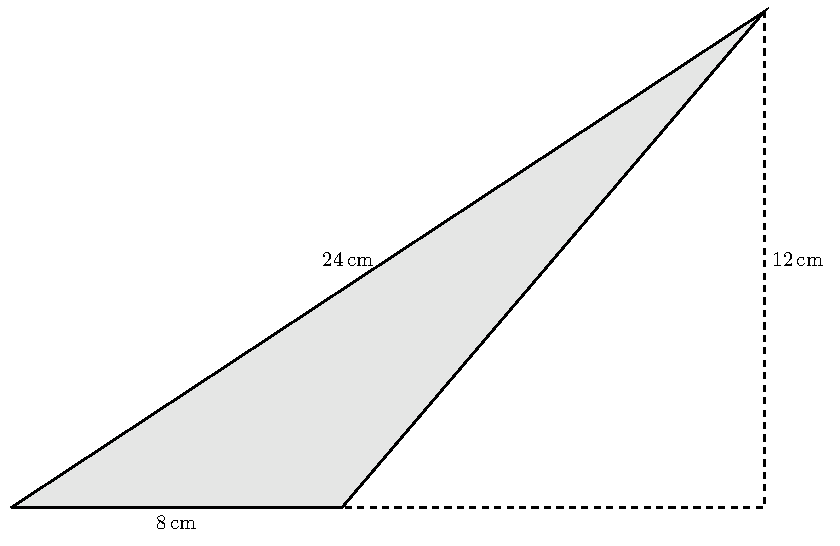
\includegraphics[height=5cm,page=1]{sprint-04-figure}
\end{center}

\begin{answer}
The base of the shaded triangle is $8$cm, the height is $12$cm, so its area is:
\begin{align*}
\frac{1}{2} \times 12 \times 8 = 48
\end{align*}
If you had not noticed that the height of the shaded triangle was $12$cm, you could have written the area of the shaded triangle as a difference of areas:
\begin{align*}
\frac{1}{2} \times 12 \times (8+x) - \frac{1}{2} \times 12 \times x = \frac{1}{2} \times 12 \times 8 = 48
\end{align*}
The unknown length $x$ cancels out of the subtraction and so it is not necessary to solve for it. 
\begin{center}
\includegraphics[height=5cm,page=2]{sprint-04-figure}
\end{center}
\begin{empheq}[box={\mathbox[colback=white]}]{equation*}
    48 ~\text{cm}^2
\end{empheq} 
\end{answer}
%%%%%%%%%%%%%%%%%%%%%%%%%%%%%%%%%%%%%%%%%%%%%%%%%%%%%%%%%%%%%%%%%%%%%%%%

\iftoggle{showAnswers}{\newpage}

%%%%%%%%%%%%%%%%%%%%%%%%%%%%%%%%%%%%%%%%%%%%%%%%%%%%%%%%%%%%%%%%%%%%%%%%
\subsection*{5.}
On Friday in Omaha, the temperature at $6{:}00$a.m. was $-3^{\circ}$F. By noon, the temperature had risen to $3^{\circ}$F. How many degrees warmer was it at noon than it was at $6{:}00$a.m.?

\nopagebreak

\fbox{\phantom{ANSWER}}~$^{\circ}$F

\begin{answer}
The temperature rose from $-3$ to $+3$, a rise in $6$ degrees. 
\begin{empheq}[box={\mathbox[colback=white]}]{equation*}
    6 ~^{\circ}\text{F}
\end{empheq} 
\end{answer}
%%%%%%%%%%%%%%%%%%%%%%%%%%%%%%%%%%%%%%%%%%%%%%%%%%%%%%%%%%%%%%%%%%%%%%%%

\iftoggle{showAnswers}{\newpage}

%%%%%%%%%%%%%%%%%%%%%%%%%%%%%%%%%%%%%%%%%%%%%%%%%%%%%%%%%%%%%%%%%%%%%%%%
\subsection*{6.}
The average length of the human tongue is $3.9$ inches. At an average length of $19$ inches, a giraffe's tongue is how many times that of a human? Express your answer to the nearest integer. 

\nopagebreak

\fbox{\phantom{ANSWER}}~times

\begin{answer}
The giraffe's tongue is $m$ times longer, where
\begin{align*}
19 & = m \times 3.9 \\
\Rightarrow m & = \frac{19}{3.9} \approx 5
\end{align*} 
\begin{empheq}[box={\mathbox[colback=white]}]{equation*}
    5 ~\text{times}
\end{empheq} 
\end{answer}
%%%%%%%%%%%%%%%%%%%%%%%%%%%%%%%%%%%%%%%%%%%%%%%%%%%%%%%%%%%%%%%%%%%%%%%%

\iftoggle{showAnswers}{\newpage}

%%%%%%%%%%%%%%%%%%%%%%%%%%%%%%%%%%%%%%%%%%%%%%%%%%%%%%%%%%%%%%%%%%%%%%%%
\subsection*{7.}
To make slime, mix $1$ ounce of school glue with $\dfrac{1}{2}$ cup of water and $\dfrac{1}{4}$ cup of sodium tetraborate. How many cups of water would be needed to make a batch of slime using $\dfrac{1}{2}$ cup of sodium tetraborate? 

\nopagebreak

\fbox{\phantom{ANSWER}}~cups

\begin{answer}
$\dfrac{1}{2}$ cup of sodium tetraborate is twice $\dfrac{1}{4}$, so the number of cups of water must be twice $\dfrac{1}{2}$ cup, or one cup.
\begin{empheq}[box={\mathbox[colback=white]}]{equation*}
    1 ~\text{cups}
\end{empheq} 
\end{answer}
%%%%%%%%%%%%%%%%%%%%%%%%%%%%%%%%%%%%%%%%%%%%%%%%%%%%%%%%%%%%%%%%%%%%%%%%

\iftoggle{showAnswers}{\newpage}

%%%%%%%%%%%%%%%%%%%%%%%%%%%%%%%%%%%%%%%%%%%%%%%%%%%%%%%%%%%%%%%%%%%%%%%%
\subsection*{8.}
If $\dfrac{1}{6}+\dfrac{1}{7}+\dfrac{1}{n}=\dfrac{1}{3}$, what is the value of $n$? 

\nopagebreak

\fbox{\phantom{ANSWER}}

\begin{answer}
\begin{align*}
\dfrac{1}{6}+\dfrac{1}{7}+\dfrac{1}{n} & = \dfrac{1}{3} \\
\Rightarrow \dfrac{1}{n} 
& = \dfrac{1}{3} - \dfrac{1}{6} - \dfrac{1}{7} 
  = \dfrac{2 \times 7 - 7 - 6}{6 \times 7} 
  = \dfrac{1}{42} \\
\Rightarrow n & = 42
\end{align*}
\begin{empheq}[box={\mathbox[colback=white]}]{equation*}
    42
\end{empheq} 
\end{answer}
%%%%%%%%%%%%%%%%%%%%%%%%%%%%%%%%%%%%%%%%%%%%%%%%%%%%%%%%%%%%%%%%%%%%%%%%

\iftoggle{showAnswers}{\newpage}

%%%%%%%%%%%%%%%%%%%%%%%%%%%%%%%%%%%%%%%%%%%%%%%%%%%%%%%%%%%%%%%%%%%%%%%%
\subsection*{9.}
Equilateral triangle $ABC$ and square $ACDE$ share side $AC$ as shown. If square $ACDE$ has area $9$m$^{2}$, what is the perimeter of pentagon $ABCDE$?

\nopagebreak

\fbox{\phantom{ANSWER}}~meters

\begin{center}
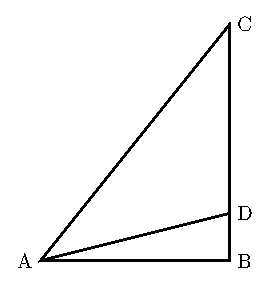
\includegraphics[height=5cm]{sprint-09-figure}
\end{center}

\begin{answer}
If $ACDE$ has area $9$m$^2$, it means the length of the edges is $3$m (since $3m \times 3m = 9m^2$). This gives a perimeter of $5 \times 3$m $=15$m. 
\begin{empheq}[box={\mathbox[colback=white]}]{equation*}
    15 ~\text{meters}
\end{empheq} 
\end{answer}
%%%%%%%%%%%%%%%%%%%%%%%%%%%%%%%%%%%%%%%%%%%%%%%%%%%%%%%%%%%%%%%%%%%%%%%%

\iftoggle{showAnswers}{\newpage}

%%%%%%%%%%%%%%%%%%%%%%%%%%%%%%%%%%%%%%%%%%%%%%%%%%%%%%%%%%%%%%%%%%%%%%%%
\subsection*{10.}
Company A sells pencils in packs of $12$ for $\$1.50$. Company B sells pencils in packs of $15$ for $\$2.00$. What is the absolute difference of the total costs to purchase $60$ pencils from each company? 

\nopagebreak

\$~\fbox{\phantom{ANSWER}}

\begin{answer}
The cost of $60$ pencils are: 
\begin{align*}
& \text{Company A:}~ 60 \times \frac{1.50}{12} 
= \frac{6 \times 15}{12} = 7.5 \\
& \text{Company B:}~ 60 \times \frac{2.00}{15} 
= \frac{6}{3} \times \frac{20}{5} = 2 \times 4 = 8 \\
& \text{Absolute Difference:}~ |8 - 7.5| = 0.5
\end{align*} 
\begin{empheq}[box={\mathbox[colback=white]}]{equation*}
    \$ 0.5
\end{empheq} 
\end{answer}
%%%%%%%%%%%%%%%%%%%%%%%%%%%%%%%%%%%%%%%%%%%%%%%%%%%%%%%%%%%%%%%%%%%%%%%%

\iftoggle{showAnswers}{\newpage}

%%%%%%%%%%%%%%%%%%%%%%%%%%%%%%%%%%%%%%%%%%%%%%%%%%%%%%%%%%%%%%%%%%%%%%%%
\subsection*{11.}
What is the smallest even integer greater than $10,000$ that contains three distinct odd digits? 

\nopagebreak

\fbox{\phantom{ANSWER}}

\begin{answer}
The smallest integer greater than $10,000$ (most likely) starts with $1$ and ends with $0$. Since $1$ is an odd digit, we are looking for another two odd digits, different from $1$, to fill the three remaining spaces: these two integers must be as small as possible, so they are $3$ and $5$. The middle digits are therefore $0$, $3$, and $5$, and must appear in that order to minimize the value, so that the integer is: $10,350$.
\begin{empheq}[box={\mathbox[colback=white]}]{equation*}
    10,350 
\end{empheq} 
\end{answer}
%%%%%%%%%%%%%%%%%%%%%%%%%%%%%%%%%%%%%%%%%%%%%%%%%%%%%%%%%%%%%%%%%%%%%%%%

\iftoggle{showAnswers}{\newpage}

%%%%%%%%%%%%%%%%%%%%%%%%%%%%%%%%%%%%%%%%%%%%%%%%%%%%%%%%%%%%%%%%%%%%%%%%
\subsection*{12.}
Sean had $\$72$ in his bank account before he spent $\dfrac{1}{4}$ of it on a birthday present for his mom. He then deposited $\$54.33$ into his bank account. How much money does Sean have in his account now?

\nopagebreak

\$~\fbox{\phantom{ANSWER}}

\begin{answer}
Let $m$ denote Sean's money. 
\begin{align*}
m & = 72 - \frac{1}{4} \times 72 + 54.33 \\
  & = \frac{3}{4} \times 72 + 54.33 \\
  & = 54 + 54.33 \\
  & = 108.33
\end{align*} 
\begin{empheq}[box={\mathbox[colback=white]}]{equation*}
    \$ 108.33
\end{empheq} 
\end{answer}
%%%%%%%%%%%%%%%%%%%%%%%%%%%%%%%%%%%%%%%%%%%%%%%%%%%%%%%%%%%%%%%%%%%%%%%%

\iftoggle{showAnswers}{\newpage}

%%%%%%%%%%%%%%%%%%%%%%%%%%%%%%%%%%%%%%%%%%%%%%%%%%%%%%%%%%%%%%%%%%%%%%%%
\subsection*{13.}
What is the fewest number of consecutive primes, starting with $2$, that when summed produce a number divisible by $7$?

\nopagebreak

\fbox{\phantom{ANSWER}}~primes

\begin{answer}
Adding consecutive primes starting with $2$ yields:
\begin{align*}
2 + 3 & = 5 < 7\\
2 + 3 + 5 & = 10 = 1 \times 7 + 3\\
2 + 3 + 5 + 7 & = 17 = 2 \times 7 + 3\\
2 + 3 + 5 + 7 + 11 & = 28 = 4 \times 7 ~\checkmark 
\end{align*} 
We need to add $2$, $3$, $5$, $7$, and $11$.
\begin{empheq}[box={\mathbox[colback=white]}]{equation*}
    5 ~\text{primes}
\end{empheq} 
\end{answer}
%%%%%%%%%%%%%%%%%%%%%%%%%%%%%%%%%%%%%%%%%%%%%%%%%%%%%%%%%%%%%%%%%%%%%%%%

\iftoggle{showAnswers}{\newpage}

%%%%%%%%%%%%%%%%%%%%%%%%%%%%%%%%%%%%%%%%%%%%%%%%%%%%%%%%%%%%%%%%%%%%%%%%
\subsection*{14.}
What is the degree measure of angle A in the figure shown here?

\nopagebreak

\fbox{\phantom{ANSWER}}~degrees

\begin{center}
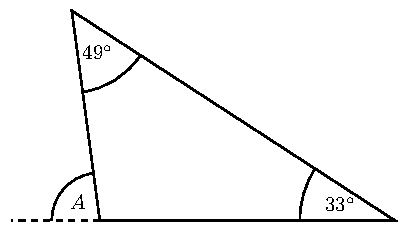
\includegraphics[height=5cm]{sprint-14-figure}
\end{center}

\begin{answer}
The angles of the triangle sum to $180^{\circ}$, so that the angle complementary to A is given by:
\begin{align*}
180 - 49 - 33 = 98
\end{align*}
and so the angle A is simply
\begin{align*}
180 - 98 = 49 + 33 = 82
\end{align*}
\begin{empheq}[box={\mathbox[colback=white]}]{equation*}
    82 ~\text{degrees}
\end{empheq} 
\end{answer}
%%%%%%%%%%%%%%%%%%%%%%%%%%%%%%%%%%%%%%%%%%%%%%%%%%%%%%%%%%%%%%%%%%%%%%%%

\iftoggle{showAnswers}{\newpage}

%%%%%%%%%%%%%%%%%%%%%%%%%%%%%%%%%%%%%%%%%%%%%%%%%%%%%%%%%%%%%%%%%%%%%%%%
\subsection*{15.}
What is the value of $(1.6+5)^2 - 1.6^2-5^2$?

\nopagebreak

\fbox{\phantom{ANSWER}}

\begin{answer}
Developing the square will clearly yields simplifications:
\begin{align*}
& (1.6+5)^2 = 1.6^2 + 2 \times 1.6 \times 5 + 5^2 \\
\Rightarrow 
& (1.6+5)^2 - 1.6^2-5^2 = 2 \times 1.6 \times 5
= 16
\end{align*}
\begin{empheq}[box={\mathbox[colback=white]}]{equation*}
    16
\end{empheq} 
\end{answer}
%%%%%%%%%%%%%%%%%%%%%%%%%%%%%%%%%%%%%%%%%%%%%%%%%%%%%%%%%%%%%%%%%%%%%%%%

\iftoggle{showAnswers}{\newpage}

%%%%%%%%%%%%%%%%%%%%%%%%%%%%%%%%%%%%%%%%%%%%%%%%%%%%%%%%%%%%%%%%%%%%%%%%
\subsection*{16.}
On a number line, what number is two-thirds of the way from $\dfrac{5}{8}$ to $\dfrac{7}{4}$? Express your answer as a common fraction.

\nopagebreak

\begin{minipage}[b]{\linewidth}
\fbox{\phantom{ANSWER}}\\
\mbox{---------------}\\
\fbox{\phantom{ANSWER}}
\end{minipage}

\begin{answer}
$\dfrac{2}{3}$ of the way from $\dfrac{5}{8}$ to $\dfrac{7}{4}$ is:
\begin{align*}
\frac{5}{8} + \frac{2}{3} \left(\frac{7}{4} - \frac{5}{8} \right)
= \frac{1}{3} \times \frac{5}{8} + \frac{2}{3} \times \frac{7}{4}
= \frac{5 + 28}{24}
= \frac{11}{8}
\end{align*}
\begin{empheq}[box={\mathbox[colback=white]}]{equation*}
    \frac{11}{8}
\end{empheq} 
\end{answer}
%%%%%%%%%%%%%%%%%%%%%%%%%%%%%%%%%%%%%%%%%%%%%%%%%%%%%%%%%%%%%%%%%%%%%%%%

\iftoggle{showAnswers}{\newpage}

%%%%%%%%%%%%%%%%%%%%%%%%%%%%%%%%%%%%%%%%%%%%%%%%%%%%%%%%%%%%%%%%%%%%%%%%
\subsection*{17.}
If the cube of a positive number is three times the square of the number, what is the number?

\nopagebreak

\fbox{\phantom{ANSWER}}~

\begin{answer}
The statement may be expressed as:
\begin{align*}
x^3 & = 3 x^2 \\
\Rightarrow x & = 3
\end{align*}
\begin{empheq}[box={\mathbox[colback=white]}]{equation*}
    3
\end{empheq} 
\end{answer}
%%%%%%%%%%%%%%%%%%%%%%%%%%%%%%%%%%%%%%%%%%%%%%%%%%%%%%%%%%%%%%%%%%%%%%%%

\iftoggle{showAnswers}{\newpage}

%%%%%%%%%%%%%%%%%%%%%%%%%%%%%%%%%%%%%%%%%%%%%%%%%%%%%%%%%%%%%%%%%%%%%%%%
\subsection*{18.}
Jan and Jerome are mixing red paint with white paint to make pink paint, in the ratio of $4$ parts red to $5$ parts white. How many gallons of red paint should they mix with $1$ gallon of white paint? Express your answer as a common fraction. 

\nopagebreak

\begin{minipage}[b]{\linewidth}
\fbox{\phantom{ANSWER}}\\
\mbox{---------------}~~gallons\\
\fbox{\phantom{ANSWER}}
\end{minipage}

\begin{answer}
The red/white mix is in ratio $4{:}5$, so there is $\dfrac{4}{5}$ for each unit of white paint.
\begin{empheq}[box={\mathbox[colback=white]}]{equation*}
    \frac{4}{5}
\end{empheq} 
\end{answer}
%%%%%%%%%%%%%%%%%%%%%%%%%%%%%%%%%%%%%%%%%%%%%%%%%%%%%%%%%%%%%%%%%%%%%%%%

\iftoggle{showAnswers}{\newpage}

%%%%%%%%%%%%%%%%%%%%%%%%%%%%%%%%%%%%%%%%%%%%%%%%%%%%%%%%%%%%%%%%%%%%%%%%
\subsection*{19.}
Tho population of Clown Town in $2020$ was $24,500$. In $2021$, the population had risen to $26,950$. What was the percent increase in population of Clown Town?

\nopagebreak

\fbox{\phantom{ANSWER}}~\%

\begin{answer}
The percent increase is:
\begin{align*}
\frac{26,950-24,500}{24,500} 
= \frac{26,950}{24,500} - 1
= 0.1
\end{align*}
\begin{empheq}[box={\mathbox[colback=white]}]{equation*}
    10 ~\%
\end{empheq} 
\end{answer}
%%%%%%%%%%%%%%%%%%%%%%%%%%%%%%%%%%%%%%%%%%%%%%%%%%%%%%%%%%%%%%%%%%%%%%%%

\iftoggle{showAnswers}{\newpage}

%%%%%%%%%%%%%%%%%%%%%%%%%%%%%%%%%%%%%%%%%%%%%%%%%%%%%%%%%%%%%%%%%%%%%%%%
\subsection*{20.}
A class meets one day a week for four weeks. The number of students in attendance at each of the four class meetings is given in the table shown. What is the sum of the mean and median number of students in attendance per week? 

\nopagebreak

\fbox{\phantom{ANSWER}}~students

\begin{center}
\renewcommand{\arraystretch}{1.5}
\rowcolors{0}{white}{gray!20}
\begin{tabular}{@{}L{3cm}C{4cm}@{}} 
\toprule
    Meeting & Attendance \\
\midrule
    Week 1 & 32 \\
    Week 2 & 27 \\
    Week 3 & 28 \\
    Week 4 & 23 \\
\bottomrule
\end{tabular}
\end{center}

\begin{answer}
Mean attendance is:
\begin{align*}
\frac{32 + 27 + 28 + 23}{4} 
= 27.5
\end{align*} 
Median attendance is:
\begin{align*}
\frac{27 + 28}{2} 
= 27.5
\end{align*} 
The sum is therefore $27.5 + 27.5 = 55$.
\begin{empheq}[box={\mathbox[colback=white]}]{equation*}
    55 ~\text{students}
\end{empheq} 
\end{answer}
%%%%%%%%%%%%%%%%%%%%%%%%%%%%%%%%%%%%%%%%%%%%%%%%%%%%%%%%%%%%%%%%%%%%%%%%

\iftoggle{showAnswers}{\newpage}

%%%%%%%%%%%%%%%%%%%%%%%%%%%%%%%%%%%%%%%%%%%%%%%%%%%%%%%%%%%%%%%%%%%%%%%%
\subsection*{21.}
What is the value of $99^2+101^2$?

\nopagebreak

\fbox{\phantom{ANSWER}}

\begin{answer}
The sum of two squares may be found from the expansion of a binomial expression. 
\begin{align*}
(99 + 101)^2 & = 99^2 + 2 \times 99 \times 101 + 101^2 \\
\Rightarrow
99^2 + 101^2 & = (99 + 101)^2 - 2 \times 99 \times 101 \\
& = 200^2 - 2 \times 9999
= 40,000 - 19,998
= 20,002
\end{align*} 
\begin{empheq}[box={\mathbox[colback=white]}]{equation*}
    20,002
\end{empheq} 
\end{answer}
%%%%%%%%%%%%%%%%%%%%%%%%%%%%%%%%%%%%%%%%%%%%%%%%%%%%%%%%%%%%%%%%%%%%%%%%

\iftoggle{showAnswers}{\newpage}

%%%%%%%%%%%%%%%%%%%%%%%%%%%%%%%%%%%%%%%%%%%%%%%%%%%%%%%%%%%%%%%%%%%%%%%%
\subsection*{22.}
Griffin bakes a perfectly circular pizza with a diameter of $10$ inches, and he sells it for $\$0.20$ per square inch. What is the cost for the entire pizza? Express your answer to the nearest whole dollar.

\nopagebreak

\$~\fbox{\phantom{ANSWER}}

\begin{answer}
The circular pizza has area:
\begin{align*}
\pi (d/2)^2 = \pi(10/2)^2 = 25\pi
\end{align*}
The total cost:
\begin{align*}
25\pi \times 0.20 = 5\pi \approx 15.71
\end{align*}
\begin{empheq}[box={\mathbox[colback=white]}]{equation*}
    \$~16
\end{empheq}
\end{answer}
%%%%%%%%%%%%%%%%%%%%%%%%%%%%%%%%%%%%%%%%%%%%%%%%%%%%%%%%%%%%%%%%%%%%%%%%

\iftoggle{showAnswers}{\newpage}

%%%%%%%%%%%%%%%%%%%%%%%%%%%%%%%%%%%%%%%%%%%%%%%%%%%%%%%%%%%%%%%%%%%%%%%%
\subsection*{23.}
What is the arithmetic mean of the first ten positive perfect squares? Express your answer as a decimal to the nearest tenth. 

\nopagebreak

\fbox{\phantom{ANSWER}}~

\begin{answer}
The sum of the first ten positive perfect squares is:
\begin{align*}
& 1^2 + 2^2 + 3^2 + 4^2 + 5^2 + 6^2 + 7^2 + 8^2 + 9^2 + 10^2 \\
& = 1 + 4 + 9 + 16 + 25 + 36 + 49 + 64 + 81 + 100 \\
& = 385
\end{align*}
And so the mean is $385/10=38.5$
\begin{empheq}[box={\mathbox[colback=white]}]{equation*}
    38.5
\end{empheq}
\end{answer}
%%%%%%%%%%%%%%%%%%%%%%%%%%%%%%%%%%%%%%%%%%%%%%%%%%%%%%%%%%%%%%%%%%%%%%%%

\iftoggle{showAnswers}{\newpage}

%%%%%%%%%%%%%%%%%%%%%%%%%%%%%%%%%%%%%%%%%%%%%%%%%%%%%%%%%%%%%%%%%%%%%%%%
\subsection*{24.}
This figure shows the floorplan of a room than includes a door and a window that have a combined area of $50$ft$^2$. Each side of the room has a wall that is $8$ feet tall, and adjacent walls meet at right angles. If a can of paint covers an area of $400$ft$^2$, how many whole cans of paint must be purchased to paint the interior walls of this room, not including the door and the window?

\nopagebreak

\fbox{\phantom{ANSWER}}~cans

\begin{center}
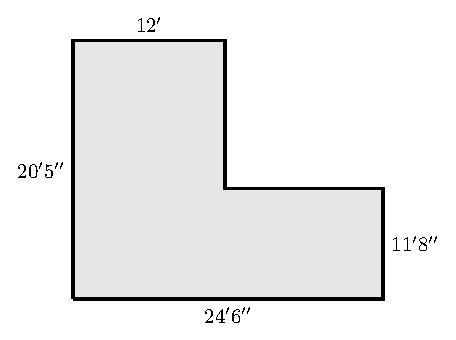
\includegraphics[height=7cm,page=1]{sprint-24-figure}
\end{center}


\begin{answer}
It is convenient to convert distances to inches: 
\begin{align*}
    8\,\text{ft} & = 96\,\text{in}\\
20\,\text{ft}\,5\,\text{in} & = 245\,\text{in}\\
24\,\text{ft}\,6\,\text{in} & = 294\,\text{in}\\
   50\,\text{ft} & = 600\,\text{in}
\end{align*}
The area of the walls (including openings) is the height multiplied by the perimeter of the room. With this particular shape, the perimeter is twice the total width and length of the figure. The area of the room in inches is therefore:
\begin{align*}
2 \times (245 + 294) \times 96  - 600
  = 102888
\end{align*}
To find how much paint is needed, we convert $400$ft$^2$ to in$^2$. One square foot is the area spanned by a square of side length $12$ inches.
\begin{center}
\includegraphics[height=6cm,page=2]{sprint-24-figure}
\end{center}
And therefore:
\begin{align*}
400\,\text{ft}^2 = 400 \times 144 = 57600\,\text{in}^2
\end{align*}
The number of cans is obtained by rounding up:
\begin{align*}
\frac{102888}{57600} = 1.78625 \rightarrow 2
\end{align*}
\begin{empheq}[box={\mathbox[colback=white]}]{equation*}
    2 ~\text{cans}
\end{empheq} 
\end{answer}
%%%%%%%%%%%%%%%%%%%%%%%%%%%%%%%%%%%%%%%%%%%%%%%%%%%%%%%%%%%%%%%%%%%%%%%%

\iftoggle{showAnswers}{\newpage}

%%%%%%%%%%%%%%%%%%%%%%%%%%%%%%%%%%%%%%%%%%%%%%%%%%%%%%%%%%%%%%%%%%%%%%%%
\subsection*{25.}
Sam has exactly $\$18.90$ in dimes and quarters, with twice as many dimes as quarters. He spends five quarters and twice as many dimes at the convenience store, and he spends $55$ cents at the donut shop. If he pays the exact amount for everything, how many quarters does Sam have left?

\nopagebreak

\fbox{\phantom{ANSWER}}~quarters

\begin{answer}
Let $d$ denote the number of dimes, and $q$ the number of quarters. A dime is worth $10$ cents, a quarter $25$ cents. We have:
\begin{align*}
10d + 25q & = 1890 \\
d & = 2 q
\end{align*}
These two equations form a linear system in $d$ and $q$. Solving for $q$ yields:
\begin{align*}
10 \times 2q + 25q & = 1890 \\
\Rightarrow
    q & = \frac{1890}{45} = 42
\end{align*}
Sam spends $5$ quarters at the convenience store, which leaves $42-5=37$ quarters. He then spends $55$ cents at the donut shop. The only way to make $55$ with dimes and quarters is to use $1$ quarter and $3$ dimes. That leaves Sam with $37-1=36$ quarters.
For the sake of completeness, consider what happens to Sam's money. Let $m$ denote the total amount of money Sam has left after spending at the convenience store and donut shop: 
\begin{align*}
m & = 1890 - 5 \times 42 - 10 \times 84 - 55 = 785~ \text{cents} = \$7.85
\end{align*}
\begin{empheq}[box={\mathbox[colback=white]}]{equation*}
    36 ~\text{quarters}
\end{empheq} 
\end{answer}
%%%%%%%%%%%%%%%%%%%%%%%%%%%%%%%%%%%%%%%%%%%%%%%%%%%%%%%%%%%%%%%%%%%%%%%%

\iftoggle{showAnswers}{\newpage}

%%%%%%%%%%%%%%%%%%%%%%%%%%%%%%%%%%%%%%%%%%%%%%%%%%%%%%%%%%%%%%%%%%%%%%%%
\subsection*{26.}
Quinn is handing a framed picture that is $10$ inches wide and $6$ inches tall on a wall that is $8$ feet $7$ inches wide and $7$ feet $4$ inches tall. When the picture is exactly centered on the wall, the left edge of the picture frame is $x$ feet $y$ inches from the left edge of the wall. What is the value of $y$, if $y<12$? Express your answer as a mixed number.

\nopagebreak

\begin{minipage}[b]{\linewidth}
\phantom{ANSWER}\hspace{14pt}\fbox{\phantom{ANSWER}}\\
\fbox{\phantom{ANSWER}}~~\mbox{---------------}\\
\phantom{ANSWER}\hspace{14pt}\fbox{\phantom{ANSWER}}

\end{minipage}

\begin{answer}
It is useful to convert feet/inches to inches and sketch a picture to scale. 
\begin{align*}
& \text{Height:}~ 7\,\text{ft}\, 4 \,\text{in}~ = 7 \times 12 + 4 = 88 \,\text{in}\\ 
& \text{Width:}~ 8\, \text{ft}\, 7 \,\text{in}~ = 8 \times 12 + 7 = 103 \,\text{in}
\end{align*}
The picture takes up $10$ inches of the $103$ width, leaving $(103-10)/2=46.5$ on either side, and $6$ inches of the $88$ height, leaving $(88-6)/2=41$ above and below. The distance between the left edge of the picture and the left edge of the wall is:
\begin{align*}
\frac{103-10}{2}
    & = 46.5 \,\text{in} \\
    & = 3 \,\text{ft} + 10\,\text{in} + \frac{1}{2}\,\text{in}\\
\Rightarrow 
  x & = 3 \,\text{ft} \\
  y & = 10\,\text{in} + \frac{1}{2}\,\text{in}
\end{align*}
\begin{center}
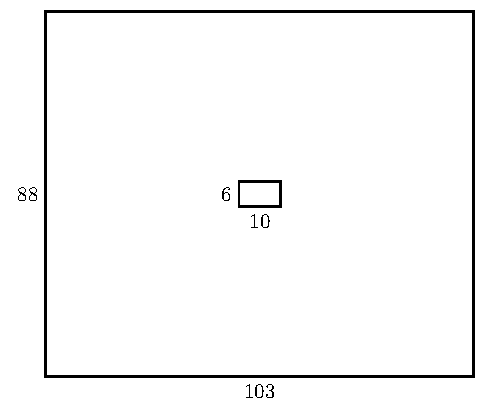
\includegraphics[height=6cm,page=1]{sprint-26-figure}
\end{center}

\begin{empheq}[box={\mathbox[colback=white]}]{equation*}
    10 \frac{1}{2}
\end{empheq} 
\end{answer}
%%%%%%%%%%%%%%%%%%%%%%%%%%%%%%%%%%%%%%%%%%%%%%%%%%%%%%%%%%%%%%%%%%%%%%%%

\iftoggle{showAnswers}{\newpage}

%%%%%%%%%%%%%%%%%%%%%%%%%%%%%%%%%%%%%%%%%%%%%%%%%%%%%%%%%%%%%%%%%%%%%%%%
\subsection*{27.}
In the figure shown, lines $m$ and $n$ are parallel, and the angle labeled $4$ measures $104$ degrees. What is the degree measure of the angle labeled $7$? 

\nopagebreak

\fbox{\phantom{ANSWER}}~degrees

\begin{center}
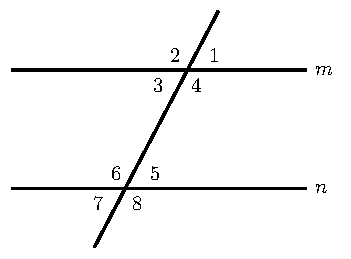
\includegraphics[height=6cm,page=1]{sprint-27-figure}
\end{center}

\begin{answer}
The angle labeled $7$ is the same as the angle labeled $3$, which is complementary with $4$, so that
\begin{align*}
\text{angle}~7 
= \text{angle}~3 
= 180 - \text{angle}~4 
= 180-104
= 76
\end{align*}
\begin{empheq}[box={\mathbox[colback=white]}]{equation*}
    76 ~\text{degrees}
\end{empheq} 
\end{answer}
%%%%%%%%%%%%%%%%%%%%%%%%%%%%%%%%%%%%%%%%%%%%%%%%%%%%%%%%%%%%%%%%%%%%%%%%

\iftoggle{showAnswers}{\newpage}

%%%%%%%%%%%%%%%%%%%%%%%%%%%%%%%%%%%%%%%%%%%%%%%%%%%%%%%%%%%%%%%%%%%%%%%%
\subsection*{28.}
In the figure, a terrenella bee moth (Aphomia terrenella) is pictured next to part of a ruler marked in centimeters. How many terrenella bee moths of equal length, placed end to end, have a combined length of $2$ meters?

\nopagebreak

\fbox{\phantom{ANSWER}}~moths

\begin{center}
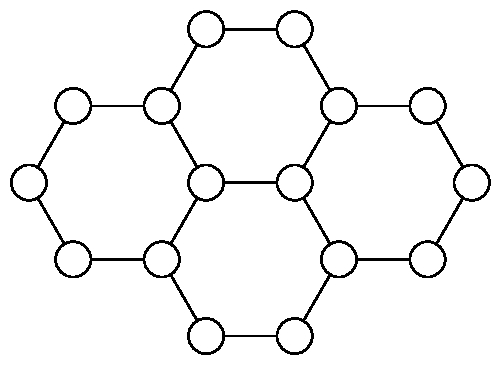
\includegraphics[height=7cm,page=1]{sprint-28-figure}
\end{center}

\begin{answer}
The moth measures $1.6$cm. There are $200$ centimeters in $2$ meters, so that 
\begin{align*}
\frac{200}{1.6} = \frac{2000}{16} = \frac{1000}{8} = \frac{500}{4} = 125
\end{align*}
\begin{empheq}[box={\mathbox[colback=white]}]{equation*}
    125 ~\text{moths}
\end{empheq} 
\end{answer}
%%%%%%%%%%%%%%%%%%%%%%%%%%%%%%%%%%%%%%%%%%%%%%%%%%%%%%%%%%%%%%%%%%%%%%%%

\iftoggle{showAnswers}{\newpage}

%%%%%%%%%%%%%%%%%%%%%%%%%%%%%%%%%%%%%%%%%%%%%%%%%%%%%%%%%%%%%%%%%%%%%%%%
\subsection*{29.}
Eli started saving money in his empty piggy bank. He inserted $\$1$ on every Monday, $\$2$ on every Tuesday, $\$3$ on every Wednesday, $\$4$ on every Thursday, $\$5$ on every Friday, $\$6$ on every Saturday, and $\$7$ on every Sunday. At the end of $24$ days, he opened his bank and found he had $\$93$. On which day of the week did he start inserting money into his piggy bank?

\nopagebreak

\fbox{\phantom{ANSWER}}

\begin{answer}
%Let $M$ stand for Monday, $T$ for Tuesday, $W$ for Wednesday, $J$ for Thursday (`jueves/jeudi'), $F$ for Friday, $S$ for Saturday, $D$ for Sunday (`domingo/dimanche'). We are looking for integers $M,T,W,J,F,S,D$ such that
%\begin{align*}
%M + 2T + 3W + 4J + 5F + 6S + 7D = 93 
%\end{align*}
%and for any two such integers $m,n$ either $m=n$ or $|m-n|=1$.
A period of $24$ days is three weeks and three days. Eli must have saved for three full weeks:
\begin{align*}
3 \times (1+2+3+4+5+6+7) = 3 \times \frac{7 \times 8}{2} = 84
\end{align*}
So we must account for $93-84 = \$9$ over $3$ days. That's not a lot of money, so it rules out the end of the week. The only way is $2+3+4=9$, Tuesday, Wednesday, Thursday. So Eli started saving on a Tuesday and opened his bank account on a Thursday. Here is a quick check:
\begin{align*}
 & \hspace{35pt}2+3+4+5+6+7 \\ 
 & +1+2+3+4+5+6+7 \\
 & +1+2+3+4+5+6+7 \\ 
 & +1+2+3+4\\
 & = 93
\end{align*}        
\begin{empheq}[box={\mathbox[colback=white]}]{equation*}
    Tuesday
\end{empheq} 
\end{answer}
%%%%%%%%%%%%%%%%%%%%%%%%%%%%%%%%%%%%%%%%%%%%%%%%%%%%%%%%%%%%%%%%%%%%%%%%

\iftoggle{showAnswers}{\newpage}

%%%%%%%%%%%%%%%%%%%%%%%%%%%%%%%%%%%%%%%%%%%%%%%%%%%%%%%%%%%%%%%%%%%%%%%%
\subsection*{30.}
In the figure shown, the cogwheel labeled A makes one revolution every $2$ seconds. How many revolutions will cogwheel B make every minute?

\nopagebreak

\fbox{\phantom{ANSWER}}~revolutions

\begin{minipage}[b]{\linewidth}
\centering
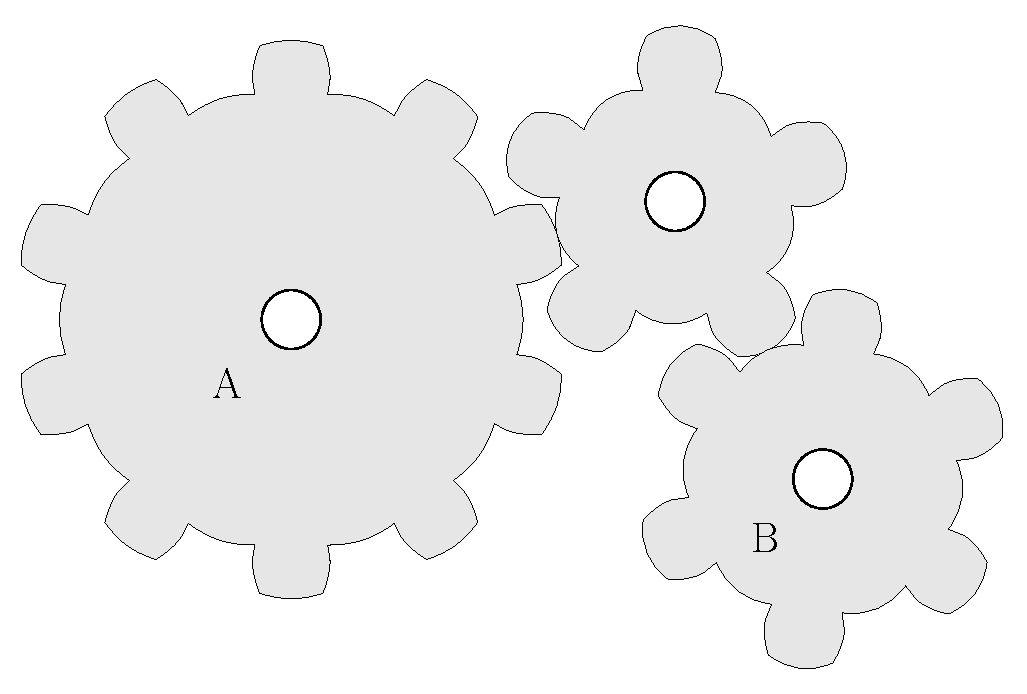
\includegraphics[height=6cm]{sprint-30-figure}
\end{minipage}

\begin{answer}
Cogwheel A makes one revolution every $2$ seconds, so $30$ times that many in one minute, since $30\times2=60$ seconds. The perimeter of each cogwheel may be measured by the number of teeth: $10$ teeth for cogwheel A vs. $6$ teeth for cogwheel B. Thus, cogwheel B goes through $10/6$th of the revolutions of cogwheel A. The revolutions of cogwheel B are therefore:
\begin{align*}
\frac{10}{6} \times 30 = 50
\end{align*}
\begin{empheq}[box={\mathbox[colback=white]}]{equation*}
    50 ~\text{revolutions}
\end{empheq} 
\end{answer}
%%%%%%%%%%%%%%%%%%%%%%%%%%%%%%%%%%%%%%%%%%%%%%%%%%%%%%%%%%%%%%%%%%%%%%%%


\end{document}